\section{Úvod do klasifikace}\label{sec:ai-uvod-klasifikace}

Klasifikace je úloha učení s~učitelem, ve které výstup není libovolné reálné číslo, ale jedna z~konečně mnoha tříd. Množinu tříd označíme
\[
    \mathcal{Y}=\set{c_1,\ldots,c_K}.
\]
Vstupní data budeme popisovat statistickými soubory
\[
    \mathbf{X}_1,\ldots,\mathbf{X}_p,
\]
výstupní třídy souborem
\[
    \mathbf{Y}=(y_1,\ldots,y_n),
    \qquad y_i\in\mathcal{Y},
\]
a~\(i\)-tý objekt vektorem
\[
    \mathbf{x}_i=(x_{i1},\ldots,x_{ip})\in\R^p.
\]

\begin{definition}\label{def:ai-klasifikator}
    \emph{Klasifikátor} je funkce
    \[
        \mapping{h}{\R^p}{\mathcal{Y}},
    \]
    která každému vektoru znaků \(\mathbf{x}\in\R^p\) přiřadí jednu třídu
    \(h(\mathbf{x})\in\mathcal{Y}\).
\end{definition}

Pro \(\mathcal{Y}=\set{0,1}\) hovoříme o~binární klasifikaci. Je-li
\(K\geqslant3\), jde o~klasifikaci vícetřídní. U~víceznačkové klasifikace může objekt nést několik značek současně; výstup pak lze zapsat vektorem z~\(\set{0,1}^K\). Dále se zaměříme hlavně na binární klasifikaci.

\subsection{Skóre, práh a~rozhodovací hranice}

Mnoho modelů nejprve vypočítá reálné skóre
\[
    \mapping{s}{\R^p}{\R}
\]
a~teprve poté z~něj určí třídu. Pro rozhodovací práh \(t\in\R\) položíme
\[
    h^{(t)}(\mathbf{x})
    =
    \begin{cases}
        1, & s(\mathbf{x})\geqslant t,\\
        0, & s(\mathbf{x})<t.
    \end{cases}
\]

\begin{definition}\label{def:ai-rozhodovaci-hranice}
    \emph{Rozhodovací hranice} skórovací funkce \(s\) při prahu \(t\) je množina
    \[
        B_t
        =
        \set{
            \mathbf{x}\in\R^p:
            s(\mathbf{x})=t
        }.
    \]
\end{definition}

\begin{figure}[ht]
    \centering
    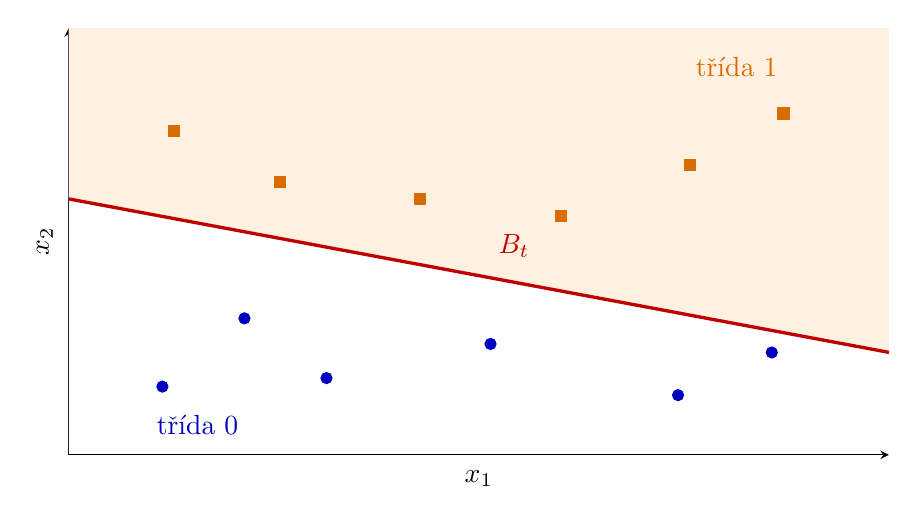
\begin{tikzpicture}
    \begin{axis}[
        width=12cm,height=7cm,
        xmin=0,xmax=7,ymin=0,ymax=5,
        axis lines=left,xlabel={$x_1$},ylabel={$x_2$},
        xtick=\empty,ytick=\empty,
        label style={font=\normalsize},
        every node/.style={font=\normalsize},
        clip=false
    ]
        \addplot[draw=none,fill=orange!12]
        coordinates{(0,3)(7,1.2)(7,5)(0,5)}\closedcycle;
        \addplot[red!75!black,very thick,domain=0:7]{3-0.257*x};
        \addplot[only marks,mark=*,blue!75!black]
        coordinates{(0.8,0.8)(1.5,1.6)(2.2,0.9)(3.6,1.3)(5.2,0.7)(6,1.2)};
        \addplot[only marks,mark=square*,orange!85!black]
        coordinates{(0.9,3.8)(1.8,3.2)(3,3)(4.2,2.8)(5.3,3.4)(6.1,4)};
        \node[red!75!black] at (axis cs:3.8,2.45){\(B_t\)};
        \node[blue!75!black] at (axis cs:1.1,0.35){třída \(0\)};
        \node[orange!85!black] at (axis cs:5.7,4.55){třída \(1\)};
    \end{axis}
\end{tikzpicture}

    \caption{Rozhodovací hranice odděluje oblasti různých předpovědí.}
    \label{fig:ai-rozhodovaci-hranice}
\end{figure}

Cílem není pouze správně klasifikovat trénovací objekty. Model má zachytit vztah mezi znaky a~třídou tak, aby správně pracoval také s~novými objekty. Příliš složitá hranice může obejít každý trénovací bod, ale na neznámých datech selhat.
